% Exercices collège: 1 \`a 42
%Il en faut 24

% Exercices  lycée:: 42 \`a 96
%Il en faut 11

% Exercices olympiques: 97 à 142
%Il en faut 9


%%%%%%%%%%%% EXERCICES COLLEGE

%1
%Eva
\begin{exo}{\nstar{0}} 
Montrer que pour tout entier $n \geq 1$, $3^{2n}-2^n$ est divisible par $7$.
\end{exo}

%2
%Eva
\begin{exo}{\nstar{0}}
Soient $a$ et $b$ deux entiers relatifs non nuls tels que les fractions $\frac{a}{600}$ et $\frac{b}{700}$ soient deux fractions irréductibles. Quel est le plus petit dénominateur possible de la fraction $\frac{7a+6b}{4200}$ ?
\end{exo}


%3
%%Matthieu Barré
\begin{exo}{\nstar{1}}
Soit $ABC$ un triangle équilatéral et $P$ un point à l'intérieur de ce triangle. Soient $D,E$ et $F$ les pieds des perpendiculaires de $P$ sur $[BC],[CA]$ et $[AB]$ respectivement. Montrer que:
\begin{enumerate}
\item $AF+BD+CE=AE+BF+CD$ et que
\item $|APF|+|BPD|+|CPE|=|APE|+|BPF|+|CPD|$,
\end{enumerate}
où $|XYZ|$ désigne l'aire du triangle $XYZ$.
\end{exo}

%4
%Giancarlo
\begin{exo}{\nstar{0}}
Soient $x,y$ deux entiers relatifs et $p$ un nombre premier. Montrer que si l'on a $x\equiv y \ [p]$ , alors on a $x^p\equiv y^p \ [p^2]$.
\end{exo}


%5
%Matthieu Barré
\begin{exo}{\nstar{0}}
Sofia dépose des grains de riz sur les cases d'un échiquier $8\times8$ de telle sorte qu'il y ait au plus un grain de riz sur chacune des $64$ cases. Déterminer le nombre maximum de grains de riz qu'elle peut placer de la sorte sans qu'il n'y ait plus de $4$ grains de riz sur une même ligne, sur une même colonne ou sur une même diagonale.
\end{exo}

%6
%Matthieu Barré
\begin{exo}{\nstar{0}}
On se donne $7$ entiers, deux à deux distincts, strictement positifs, dont la somme vaut $100$. Montrer que l'on peut en trouver trois dont la somme est au moins $50$.
\end{exo}

%7
%Matthieu Barré
\begin{exo}{\nstar{0}} Dans la pièce du milieu, $2016$ torches sont entreposées, toutes éteintes. C'est alors que Llawgad débarque, et décide de s'amuser avec. Alors, exubérant comme un gamin des rues, il commence par allumer toutes les torches. Puis il éteint les torches de numéro pair. Puis il change l'état de toutes les torches portant un numéro multiple de $3$, puis de toutes celles au numéro multiple de $4$, et ainsi de suite jusqu'à changer l'état de toutes les lampes de numéro multiple de $2016$. \`A la fin de son massacre, quelles lampes seront encore allumées ?
\end{exo}

%Matthieu Barré
%8
\begin{exo}{\nstar{1}}
Trouver tous les entiers relatifs $x$ et $y$ tels que \[x^2y+7x=x^2+3xy+3y+4.\]
\end{exo}

%9
%Matthieu Barré
\begin{exo}{\nstar{0}} 
Les nombres de $1$ à $n$ sont écrits au tableau. \`A chaque étape, on choisit deux nombres $a$ et $b$ distincts du tableau, on les efface puis on les remplace par $ab+a+b$, et on réitère ce processus. Quel sera le dernier nombre écrit au tableau ?
%vide
\end{exo}

%10
\begin{exo}{\nstar{3}}Soit $[EF]$ un segment inclus dans le segment $[BC]$ tel que le demi-cercle de diamètre $[EF]$ est tangent à $[AB]$ en $Q$ et à $[AC]$ en $P$. Prouver que le point d'intersection $K$ des droites $(EP)$ et $(FQ)$ appartient à la hauteur issue de $A$ du triangle $ABC$.
\end{exo}

%11
%Matthieu Barré
\begin{exo}{\nstar{0}}
Soient $a$ et $b$ deux nombres réels et $f$ la fonction de $\mathbb{R}$ dans $\mathbb{R}$ qui à $x$ associe $x^2+ax+b$. On suppose  qu'il existe un réel $t$ tel que $f(t)=f(f(f(t)))=0$. Montrer que $f(0) \times f(1)=0$.
\end{exo}

%12
%Matthieu Barré
\begin{exo}{\nstar{0}}
Combien y a-t-il d'entiers positifs $n$ tels que
\[\frac{n^{2016}}{n-2016}\]
soit un nombre entier ?
\end{exo}

%Nicolas
%13
\begin{exo}{\nstar{1}}Soit $ABC$ un triangle. Soit $I$ un point du segment $[AB]$. Montrer que la droite $(CI)$ est la bissectrice intérieure issue de $C$ si et seulement si $CA/CB=IA/IB$.
\end{exo}

%14
\begin{exo}{\nstar{2}}
Montrer que $\sqrt{2}+\sqrt{5}+\sqrt{13}$ est irrationnel.
\end{exo}

%Gabriel
%15
\begin{exo}{\nstar{1}}
Montrer que tous les termes de la suite $\left(a_{n}\right)$ définie par 
\[\begin{cases}
a_{1}=a_{2}=a_{3}=1\\
a_{n+1}=\frac{1+a_{n-1}a_{n}}{a_{n-2}}
\end{cases}\]
sont des entiers. 
\end{exo}

%16
%Matthieu Barré
\begin{exo}{\nstar{0}}
On considère $101$ points, placés à l'intérieur d'un carré $10\times10$. Montrer qu'il existe un triangle parmi les $101$ points avec une aire inférieure ou égale à $1$.
\end{exo}

%Gabriel
%17
\begin{exo}{\nstar{1}}
 Existe-t-il une
suite $\left(u_{n}\right)_{n \geq 1}$ d'entiers naturels non nuls telle que pour tous entiers $m,n \geq 1$
$u_{n}$ et $u_{m}$ sont premiers entre eux si et seulement si $\left|n-m\right|=1$
?
\end{exo}

%18
%Matthieu
\begin{exo}{\nstar{0}} 
Soit $ABC$ un triangle isocèle en $A$ et $D$ le pied de la bissectrice intérieure issue de $B$. On suppose que $BC=AD+DB$. Combien vaut $\widehat{BAC}$ ?
\end{exo}

%19
%Matthieu
\begin{exo}{\nstar{0}}
$20$ enfants sont attendus par leurs grands-pères à la sortie de l’école primaire.
On suppose que deux enfants quelconques choisis parmi les $20$ ont au moins un grand-père en commun.
Montrer qu’il y a au moins un grand-père qui attend au moins $14$ de ses petits-enfants.
\end{exo}

%Guillaume
%20
\begin{exo}{\nstar{2}}
Trouver les entiers naturels $n$ tels que $n^4+4^n$ soit premier. 
\end{exo}

%21
%Cécile
\begin{exo}{\nstar{0}}
Athalie et Bérénice jouent à un jeu. Elles prennent un cube, et tour à tour, elles en choisissent trois arêtes qu'elles colorient (Athalie en rouge, Bérénice en bleu). Le but de chaque joueuse est de colorier avant l'autre quatre arêtes d'une même face.

Athalie commence. A-t-elle une stratégie gagnante ?
\end{exo}

%22
\begin{exo}{\nstar{3}}
Trouver les entiers strictement positifs $a$ et $b$ tels que
$\frac{a^{2b+1} b-1}{a+1}$ et $\frac{b^a a+1}{b-1}$ soient des
entiers.
\end{exo}

%23
%Cécile
\begin{exo}{\nstar{0}}
Matthieu fabrique des puzzles de forme carrée. Malheureusement, il ne sait découper que des pièces carrées. Pour chaque puzzle, il prépare une boîte contenant les pièces nécessaires à la reconstitution du puzzle, et sur chaque boîte, il indique le nombre de pièces qu'elle contient.

Quel est l'ensemble des nombres qu'on peut lire sur les boîtes ?
\end{exo}


%24
\begin{exo}{\nstar{3}}
Soient $m,n$ des entiers positifs. À quelle condition existe-t-il un entier positif $N$
tel que pour tout entier $r \geq N$ il existe deux entiers positifs $a$ et $b$ tels que  $r=am+bn$ ? Estimer la valeur minimale de $N$ aussi précisément que possible.
\end{exo}

%25
%Cécilé
\begin{exo}{\nstar{0}}
Soit $ABCD,ECGF$ deux carrés tels que $B,C,G$ sont alignés et $A,D,E,F$ sont
du même côté de la droite $(BC)$. Soit $M$ l'autre point d'intersection des cercles
circonscrits à $ABCD$ et à $ECGF$.

Donner une autre construction du point $M$, n'utilisant qu'une règle non graduée.
\end{exo}

%26
%Giancarlo
\begin{exo}{\nstar{0}}
Quel est le reste de la division euclidienne de $2016^{2017^{2018}}$ par $11$ ?
\end{exo}

%27
%Victor
\begin{exo}{\nstar{0}}
Alice et Bob jouent au jeu suivant:
Alice part du nombre $2$ et les joueurs jouent chacun leur tour. 
A chaque tour, en notant $n$ le nombre atteint par le joueur précédent, on ajoute un nombre $m$ tel que $m$ divise $n$, $m \neq n$, et $m+n \leq 2016$.
Le premier joueur à ne plus pouvoir jouer a perdu.
Quel joueur peut s'assurer la victoire?
\end{exo}

%28
\begin{exo}{\nstar{4}}
Soit $ABC$ un triangle isocèle en $C$. On considère un point $P$ sur le cercle circonscrit au triangle $ABC$ situé entre $A$ et $B$ (et $P$ n'est pas du même côté que $C$ par rapport à la droite $(AB)$). Soit $D$ un point de la droite $(PB)$ tel que les droites $(CD)$ et $(PB)$ soient perpendiculaires. Prouver que
\[PA+PB= 2 \cdot PD.\]
\end{exo}

%29
\begin{exo}{\nstar{4}}
Soient $x,y>0$, et soit $s=\min(x,y+\frac1x,\frac1y)$. Quelle est la valeur maximale possible de $s$ ? Pour quels $x,y$ est-elle atteinte ?
\end{exo}

%30
%Vincent
\begin{exo}{ \nstar{0}}
Soit $f : \mathbb{R} \mapsto \mathbb{R}$ une fonction telle que $f(x+y) \geq f(xy)$ pour tous les réels $x$, $y$.
Montrer que $f$ est constante.
\end{exo}

%31
%Vincent
\begin{exo}{\nstar{0}}
Soit $ABC$ un triangle isocèle en $B$, puis $F$ un point sur la bissectrice de $\widehat{ABC}$ tel que $(AF)$ soit parallèle à $(BC)$.
Enfin, soit $E$ le milieu de $[BC]$, et soit $D$ le symétrique de $A$ par rapport à $F$.
Calculer le rapport des distances $EF / BD$.
\end{exo}

%32
\begin{exo}{\nstar{4}}
Soit $\mathcal{P}=A_1\ldots A_{2n}$ un $2n-$gone convexe dans le plan. Soit $P$ un point intérieur à $\mathcal{P}$, non situé sur une diagonale. Prouver que $P$ est contenu dans un nombre pair de triangles à sommets parmi les $A_i$.
\end{exo}

%33
%Vincent
\begin{exo}{\nstar{0}}
On écrit dans l'ordre croissant l'ensemble des entiers naturels dont l'écriture en base $1$0 ne comprend que les chiffres $2$, $0$, $1$ et $6$. Par exemple, cette suite commence par $0, 1, 2, 6, 10, 11, 12, \ldots$. En quelle position se trouve l'entier 2016 ? Quel entier se trouve en 2016\textsuperscript{ème} position ?
\end{exo}

%34
%Vincent
\begin{exo}{\nstar{0}}
On divise la figure

\[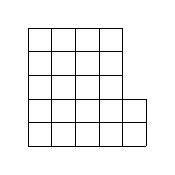
\begin{tikzpicture}[scale=0.3]
\draw (0, 0)--(0,5 );
\draw (1, 0)--(1,5 );
\draw (2, 0)--(2,5 );
\draw (3, 0)--(3,5 );
\draw (4, 0)--(4,5 );
\draw (5, 0)--(5,2 );

\draw(0,0)--(5,0);
\draw(0,1)--(5,1);
\draw(0,2)--(5,2);
\draw(0,3)--(4,3);
\draw(0,4)--(4,4);
\draw(0,5)--(4,5);
\end{tikzpicture}\]

en morceaux de forme 
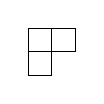
\begin{tikzpicture}[scale=0.3]
\draw(0,0)--(0,2);
\draw(1,0)--(1,2);
\draw(2,1)--(2,2);
\draw(0,0)--(1,0);
\draw(0,1)--(2,1);
\draw(0,2)--(2,2);
\end{tikzpicture}
et
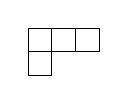
\begin{tikzpicture}[scale=0.3]
\draw(0,0)--(0,2);
\draw(1,0)--(1,2);
\draw(2,1)--(2,2);
\draw(3,1)--(3,2);
\draw(0,0)--(1,0);
\draw(0,1)--(3,1);
\draw(0,2)--(3,2);
\end{tikzpicture}.

Combien a-t-on utilisé de morceaux de forme
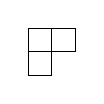
\begin{tikzpicture}[scale=0.3]
\draw(0,0)--(0,2);
\draw(1,0)--(1,2);
\draw(2,1)--(2,2);
\draw(0,0)--(1,0);
\draw(0,1)--(2,1);
\draw(0,2)--(2,2);
\end{tikzpicture} ?
\end{exo}


%35
%Vincent
\begin{exo}{\nstar{0}}
Alice a dessiné quatre pentagones, comme ci-dessous, puis a placé chacun des entiers $1, 2, \ldots, 20$
sur un sommet d'un des pentagones, de manière à ce que deux entiers distincts soient placés en deux sommets distincts.
Montrer qu'il existe nécessairement deux entiers $i$ et $j$ placés en deux sommets voisins l'un de l'autre et tels que $|i-j| \geq 4$.

Par exemple, dans le cas ci-dessous, les entiers $1$ et $5$ sont placés en deux sommets voisins,
et on a bien $|1-5| \geq 4$.

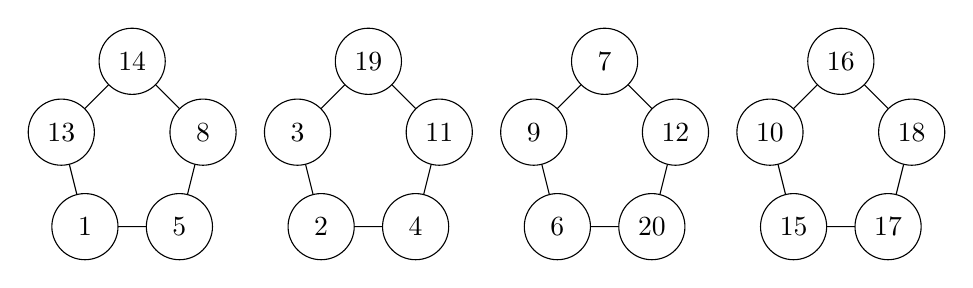
\begin{tikzpicture}[scale=0.3]
\draw (1, 2)--(0,6) -- (3,9) -- (6,6) -- (5,2) -- cycle;
\draw (11, 2)--(10,6) -- (13,9) -- (16,6) -- (15,2) -- cycle;
\draw (21, 2)--(20,6) -- (23,9) -- (26,6) -- (25,2) -- cycle;
\draw (31, 2)--(30,6) -- (33,9) -- (36,6) -- (35,2) -- cycle;
\draw[fill=white] (1,2) circle (1.4);
\draw[fill=white] (0,6) circle (1.4);
\draw[fill=white] (3,9) circle (1.4);
\draw[fill=white] (6,6) circle (1.4);
\draw[fill=white] (5,2) circle (1.4);
\node at (1,2) {1};
\node at (0,6) {13};
\node at (3,9) {14};
\node at (6,6) {8};
\node at (5,2) {5};
\draw[fill=white] (11,2) circle (1.4);
\draw[fill=white] (10,6) circle (1.4);
\draw[fill=white] (13,9) circle (1.4);
\draw[fill=white] (16,6) circle (1.4);
\draw[fill=white] (15,2) circle (1.4);
\node at (11,2) {2};
\node at (10,6) {3};
\node at (13,9) {19};
\node at (16,6) {11};
\node at (15,2) {4};
\draw[fill=white] (21,2) circle (1.4);
\draw[fill=white] (20,6) circle (1.4);
\draw[fill=white] (23,9) circle (1.4);
\draw[fill=white] (26,6) circle (1.4);
\draw[fill=white] (25,2) circle (1.4);
\node at (21,2) {6};
\node at (20,6) {9};
\node at (23,9) {7};
\node at (26,6) {12};
\node at (25,2) {20};
\draw[fill=white] (31,2) circle (1.4);
\draw[fill=white] (30,6) circle (1.4);
\draw[fill=white] (33,9) circle (1.4);
\draw[fill=white] (36,6) circle (1.4);
\draw[fill=white] (35,2) circle (1.4);
\node at (31,2) {15};
\node at (30,6) {10};
\node at (33,9) {16};
\node at (36,6) {18};
\node at (35,2) {17};
\end{tikzpicture}
\end{exo}

%36
%Vincent
\begin{exo}{\nstar{0}} 
Soit $ABC$ un triangle, $I$ le centre du cercle inscrit dans $ABC$, $D$ le pied de la hauteur de $ABI$ issue de $B$,
et $E$ le pied de la hauteur de $BCI$ issue de $B$.
Montrer que $AB = BC$ si et seulement si $BD = BE$.
\end{exo}


%37
\begin{exo}{\nstar{4}}
Soit $ABC$ un triangle isocèle en $A$ tel que $\widehat{BAC}<60^{\circ}$. Les points $D$ et $E$ sont des points du côté $[AC]$ tels que $EB=ED$ et $\widehat{ABD}=\widehat{CBE}$. Soit $O$ le point d'intersection des bissectrices des angles $\widehat{BDC}$ and $\widehat{ACB}$. Trouver la valeur de l'angle $\widehat{COD}$.
\end{exo}

%38
\begin{exo}{\nstar{4}}Trouver tous les entiers positifs $a,b,c$ tels que $$ 2^{a}3^{b}+9 = c^{2}.$$
\end{exo} 

%39
\begin{exo}{\nstar{4}} Soit $ABC$ un triangle dont tous les angles sont aigus. On note $ \Gamma$ son cercle circonscrit. On suppose que La tangente en $A$ à $\Gamma$ coupe la droite $(BC)$ en un point $P$. Soit $M$ le milieu de $[AP]$ et soit $R$ le deuxième point d'intersection de la droite $(BM)$ avec le cercle $ \Gamma$. La droite $(PR)$ recoupe le cercle $ \Gamma$ en $S$.

Prouver que les droites $(AP)$ et $(CS)$ sont parallèles.
\end{exo}


%Eva
%40
\begin{exo}{\nstar{0}} 
 \`A Mathland, deux villes sont toujours reliées soit par avion soit par bateau. Montrer qu'il est possible de choisir un moyen de transport qui permette d'aller de n'importe quelle ville à n'importe quelle autre (éventuellement avec des escales).
 \end{exo}

%Romain
%41
\begin{exo}{\nstar{0}} On considère un damier carré de côté $2n+1$. Montrer qu'il est impossible de trouver un chemin passant une unique fois sur chaque case (qui emprunte les côtés des petits carrés) et finissant sur la case initiale.
%vide
\end{exo}


%42
%Eva
\begin{exo}{\nstar{0}} 
Combien vaut la fraction continue $1+\dfrac{1}{2+\dfrac{1}{2+\dfrac{1}{\cdots}}}$ ?
\end{exo}



%%%%%%%%% Exos seconde-premiére %%%%%%%%%%%

%Matthieu Barré
%43
\begin{exo}{\nstar{1}}
Existe-t-il un triangle rectangle ayant des côtés de longueur rationnelle et dont l'aire vaut $1$ ?
\end{exo}

%Matthieu Barré
%44
\begin{exo}{ \nstar{1}}
Soit $\mathcal{P}$ la parabole d'équation $y=x^2$. Trouver une condition nécessaire et suffisante pour que des points de $\mathcal{P}$ d'abscisse $a$, $b$, $c$ et $d$ soient cocycliques.
\end{exo}

%Guillaume
%45
\begin{exo}{\nstar{2}}
Pour quels entiers $n \geq 1$ existe-t-il une bijection
\[\sigma : \{ 1,2, \ldots,n\} \rightarrow \{ 1,2, \ldots,n\},\]
de sorte que $\vert \sigma(i)-i \vert \neq \vert \sigma(j)-j \vert$ si $i \neq j$?
\end{exo}

%46
\begin{exo}{\nstar{3}}
Consid\'erons un triangle $ABC$ tel que $AB=BC$ et $\widehat{ABC} = 80^\circ$. Soit $P$ le point de l'int\'erieur de $ABC$ tel que $\widehat{PAC} = 40^\circ$ et $\widehat{PCA} = 30^\circ$. Calculer l'angle $\widehat{BPC}$.
\end{exo}

%47
\begin{exo}{ \nstar{0}}
Quel est l'entier $n$ minimal tel que, si on place $n$ points sur le
réseau hexagonal, il existe forcément deux de ces points dont le milieu est sur
le réseau hexagonal ?
\end{exo}

%48
\begin{exo}{\nstar{3}}
On considère un triangle acutangle $ABC$ avec $\widehat{A}=60^\circ$. Déterminer les points $M\in (AB)$ et $N\in (AC)$ qui minimisent la somme
\[|CM|+|MN|+|BN|.\]
\end{exo}

%Gabriel
%49
\begin{exo}{\nstar{1}}
Soit $P$ un point de l'espace
et $r>0$. Montrer qu'il existe $8$ sphères disjointes de même rayon
$r$ qui cachent le point $P$, c'est-à-dire que toute demi-droite
issue de $P$ rencontre au moins l'une des sphères. On supposera que
les centres des sphères sont tous à des distances $>r$ de $P$.

\end{exo}

%Gabriel
%50
\begin{exo}{\nstar{1}}
Parmi les quadrilatères de côtés
$a$,$b$,$c$,$d$ caractériser géométriquement celui qui a la plus
grande aire.
\end{exo}

%51
\begin{exo}{ \nstar{0}}
Achille et Briséis ont un tas de $2n+1$ jetons. Tour à tour, ils peuvent en retirer un nombre au choix entre $1$ et $2k+1$, et ce jusqu'à épuisement du tas. Le but de chaque joueur est de finir en ayant retiré, en tout, 
un nombre pair de jetons.

Achille commence. A-t-il une stratégie gagnante ?
\end{exo}

%Matthieu Barré
%52
\begin{exo}{\nstar{1}}
Soit $P$ un point à l'intérieur d'un cercle de rayon $R$, $d$ une droite passant par $P$ et $d'$ la perpendiculaire à $d$ en $P$. On fait tourner les droites $d$ et $d'$ d'un angle $\phi$ autour de $P$. Montrer que quelle que soit la position du point $P$, l'aire balayée par $d$ et $d'$ à l'intérieur du cercle (qui a la forme d'une croix) vaudra $\pi R^2 \frac{4\phi}{360}$.
\end{exo}

%Guillaume
%53
\begin{exo}{\nstar{2}}Trouver toutes les fonctions $f : \R \rightarrow \R$ telles que pour tous réels $x,y,z,t$,
$$(f(x)+f(y))(f(z)+f(t))=f(xz+yt)+f(xt-yz).$$
\end{exo}

%54
\begin{exo}{\nstar{3}}
Soit $ABC$ un triangle, $D$ le milieu de $[AB]$, $M$ le milieu de $[CD]$. On suppose
que les droites $(BM)$ et $(AC)$ sont sécantes, en un point que l'on nomme $N$.
Enfin, soit $\Gamma$ le cercle circonscrit au triangle $BCN$.
Montrer que $AB$ est tangente à $\Gamma$ si et seulement si $$\frac{BM}{MN}
= \frac{(BC)^2}{(BN)^2}.$$
\end{exo}


%55
%Gabriel
\begin{exo}{\nstar{0}}
Sophie choisit au hasard un polynôme $P$
dont tous les coefficients sont des entiers naturels. Thomas a le
droit de demander à Sophie la valeur prise par $P$ en un nombre $a$
donné, puis, en tenant éventuellement compte de la première réponse
de Sophie, en un autre nombre $b$. Thomas doit ensuite deviner le
polynôme $P$. Comment faire ? 
\end{exo}

%56
%Eva
\begin{exo}{\nstar{0}}
Peut-on trouver deux rationnels $a$ et $b$ tels qu'un carré de côté $a$ ait même aire qu'un triangle équilatéral de côté $b$ ?
\end{exo}



%Gabriel
%57
\begin{exo}{\nstar{1}}
Alice et Bob sont complices et opposés à
Eve. Dans une salle est disposé un échiquier 
avec sur chaque case une pièce de monnaie en position pile ou face.
Au départ, seuls Eve et Bob sont dans la pièce ; ce dernier observe
Eve retourner l'une des pièces. Ensuite, Eve s'en va et Bob a le droit
de retourner au plus une pièce avant de partir lui aussi. Finalement,
Alice entre dans la salle. Elle observe l'échiquier et doit déterminer
la pièce retournée par Eve. Expliquer comment Alice et Bob peuvent
se concerter à l'avance pour qu'Alice retrouve à coup sûr la pièce
retournée par Eve.
\end{exo}


%Guillaume
%58
\begin{exo}{\nstar{2}}Soit $ABC$ un triangle rectangle isocèle en $C$, $D$ et $E$ des points de $[AC]$ et $[BC]$ tels que $CE=CD$. Les perpendiculaires à $(AE)$ passant par $D$ et $C$ coupent $(AB)$ respectivement en $K$ et $L$. Montrer que $KL=LB$.
\end{exo}


%59
\begin{exo}{\nstar{2}}Démontrer que pour tout nombre réel $x \in ]0, \pi/2[$ on a l'inégalité suivante:
$$ \left( 1+ \frac{1}{\cos^{10}(x)} \right)  \left( 1+ \frac{1}{\sin^{10}(x)} \right) \geq 1089.$$
\end{exo}

%Gabriel
%60
\begin{exo}{\nstar{1}}
On considère $n$ entiers $a_{1},\ldots a_{n}$
dans $\left\{ 1,\ldots2015\right\} $ tels que le ppcm de deux d'entre
eux est toujours $>2015$. Montrer que 
\[
\frac{1}{a_{1}}+\cdots+\frac{1}{a_{n}}<2.
\]
\end{exo}

%Margaret
%61
\begin{exo}{\nstar{2}}Déterminer tous les couples de polynômes non constants $P$ et $Q$ unitaires, de degré $n$ et admettant $n$ racines positives ou nulles (non nécessairement distinctes) tels que
$$P(x) - Q(x) = 1.$$
\end{exo}

%62
%Victor
\begin{exo}{\nstar{0}}
 Dans un royaume, il y a $n$ villages et $n$ puits (non alignés). Le prince doit attribuer à chaque village son puit, en vérifiant que le segment reliant chaque village à son puit n'en croise pas d'autres. Montrer que le prince peut réussir.
\end{exo}

%Margaret
%63
\begin{exo}{\nstar{2}}On se donne un nombre entier $n>1$. Deux joueurs $R$ et $B$ colorient tour à tour des points sur un cercle, $R$ coloriant en rouge et $B$ en bleu. Une fois que chacun a placé $n$ points, le jeu s'arrête, et chaque joueur cherche sur le cercle l'arc de cercle le plus long ayant pour extrémités des points de sa couleur, et ne contenant aucun autre point coloré. Le joueur dont l'arc de cercle sélectionné est le plus long gagne (s'ils sont de même longueur, ou bien s'il n'y a aucun tel arc, on dit que la partie est nulle). L'un des deux joueurs a-t-il une stratégie gagnante?
\end{exo}

%Margaret
%64
\begin{exo}{\nstar{2}}Pour chaque nombre premier $p$, trouver le plus grand entier $k$ tel que $(p!)^k$ divise $(p^2)!$.
\end{exo}

%Margaret
%65
\begin{exo}{\nstar{2}}Soit $a_1,a_2,\ldots$ une suite infinie strictement croissante d'entiers naturels telle que pour tout $n$, le terme $a_n$ soit égal soit à la moyenne arithmétique, soit à la moyenne géométrique des deux termes $a_{n-1}$ et $a_{n+1}$. Cette suite est-elle nécessairement toujours arithmétique ou toujours géométrique à partir d'un certain rang?
\end{exo}

%Margaret
%66
\begin{exo}{\nstar{2}}On partitionne un carré en un nombre fini (supérieur à 2) de rectangles de côtés parallèles aux côtés du carré. Parmi les segments joignant les centres de deux rectangles de la partition, en existe-t-il toujours un n'intersectant aucun autre rectangle?
\end{exo}


%67
\begin{exo}{\nstar{0}}
Soit $ABCD$ un carré et soient $P,Q$ des points sur les segments $[AB],[BC]$ tels que $AP=BQ$.

\`A l'aide d'une règle non graduée, construire la perpendiculaire à $(PQ)$ passant par $D$.
\end{exo}

%68
\begin{exo}{\nstar{1}}
Soit $x_0, x_1, x_2, \ldots $ une suite de nombres réels. On dit que la suite $x_0, x_1, \ldots$ est convexe si :
\[
\frac{x_{n-1}+x_{n+1}}{2}\geq x_n\quad \textrm {pour tout entier } n \geq 0
\]
et qu'elle est log-convexe si :
\[
x_{n+1}x_{n-1}\geq x_n^2\quad \textrm {pour tout entier } n \geq 0
\]
 On suppose que pour tout nombre réel $a>0$, la suite $x_0, a x_1, a^2 x_2^2, a^3 x_3^3, \ldots$ est convexe. Prouver que la suite $x_0, x_1, \ldots $ est log-convexe.
\end{exo}



%Gabriel
%69
\begin{exo}{\nstar{1}}
Soient $a$, $b$ et $c$ les longueurs
des côté d'un triangle. Montrer que 

\[
a^{2}b\left(a-b\right)+b^{2}c\left(b-c\right)+c^{2}a\left(c-a\right)\geqslant0
\]
Quel est le cas d'égalité ? 
\end{exo}

%Matthieu Barré
%70
\begin{exo}{\nstar{1}}
Soit $ABC$ un triangle équilatéral de côté $a$ et $P$ un point à l'intérieur de ce triangle. On construit un triangle $XYZ$ de côtés de longueur $PA$, $PB$ et $PC$ et on note $F$ son point de Fermat. Montrer que $FX+FY+FZ=a$.
\end{exo}

%71
\begin{exo}{\nstar{3}}
Une droite passant par un point $A$ coupe un cercle $ \mathcal{C}$ en $B$ et $C$. On suppose que $B$ est situé entre $A$ et $C$. Les deux tangentes à $ \mathcal{C}$ passant par $A$ sont tangentes à $ \mathcal{C}$ en $S$ et en $T$. On note $P$ le point d'intersection de $(ST)$ et $(AC)$. Montrer que 
$ \frac{AP}{PC}=2\frac{AB}{BC} $

\end{exo}

%Guillaume
%72
\begin{exo}{\nstar{2}}Trouver toutes les fonctions $f$ de $ \N$ dans $ \N$ telles que pour tous entiers $m,n \geq 0$ on ait
$$f(m+f(n))=f(f(m))+f(n).$$
\end{exo}

%73
%Romain
\begin{exo}{\nstar{0}}
On considère l'ensemble $ \{1,2, \ldots,n\} $ dans lequel on choisit un sous-ensemble $X$. On choisit ensuite un sous-ensemble $Y$ de $X$ ainsi qu'un sous-ensemble $Z$ du complémentaire de $X$. Combient y a-t-il de choix possibles de triplets $(X, Y, Z)$?
\end{exo}



%74
\begin{exo}{\nstar{3}}
Soit $ABC$ un triangle dont le cercle inscrit est noté $ \omega$. Soient $I$ le centre  de $ \omega$ et $P$ un point tel que les droites $(PI)$ et $(BC)$ soient perpendiculaires et les droites $(PA)$ et $(BC)$ parallèles. Soient finalement $Q$ et $R$ deux points tels que $Q \in (AB)$, $R \in (AC)$, les droites $(QR)$ et $(BC)$ soient parallèles et finalement $(QR)$ soit tangente à $ \omega$.

Prouver que $ \widehat {QPB}= \widehat {CPR}$.
\end{exo}

%75
%Eva
\begin{exo}{\nstar{0}}
Un carreleur a des carreaux de taille $2 \times 1$ (ou $1 \times 2$) de deux couleurs différentes. De combien de manières possibles peut-il carreler un rectangle de taille $2 \times n$ ?
\end{exo}

%76
\begin{exo}{\nstar{0}}
On trace un grand triangle $ABC$, et on le pave avec des triangles. On 
étiquette ensuite les sommets créés de la façon suivante : à chaque 
sommet appartenant au côté $[AB]$ du grand triangle est attribuée
une lettre, $A$ ou $B$ ; à chaque sommet appartenant au côté $[BC]$ 
du grand triangle est attribué un $B$ ou un $C$ ; à chaque sommet 
appartenant au côté $[CA]$ du grand triangle est attribué un $C$ ou un $A$.
On étiquette les sommets situés strictement à l'intérieur du grand triangle
avec un $A$, un $B$ ou un $C$ au choix.

Montrer qu'on peut trouver un triangle (hormis le grand triangle) étiqueté $ABC$.
 \end{exo}


%77
\begin{exo}{\nstar{3}}
Trouver tous les polynômes $P(x)$ à coefficients réels tels que 
$$x P \left( \frac{y}{x} \right)+y P \left( \frac{x}{y} \right)=x+y$$
pour tous nombres réels non nuls $x,y$.
\end{exo}

%78
%Eva
\begin{exo}{\nstar{0}}
Existe-t-il une suite d'entiers $(u_n)_{n \in \mathbb{N}^{\star}}$ strictement croissante telle que pour tous entiers naturels $n, m$ on ait $u_{n \times m} = u_n + u_m$ ?
\end{exo}


%79
\begin{exo}{\nstar{3}}
Trouver tous les nombres premiers $p,q$ tels que $ p^2-pq-q^3=1 $.
\end{exo}

%80
%Eva
\begin{exo}{\nstar{0}}
Montrer que pour tous $a, b, c$ réels strictement positifs on a : \[ \frac{(a+2b+3c)^2}{a^2+2b^2+3c^2} \leq 6
\].
\end{exo}

%%Matthieu Barré
%81
\begin{exo}{\nstar{1}}
Trouver tous les polynômes $P$ à coefficients réels tels que, pour tout $n \in \mathbb{N}$, il existe un rationnel $r$ tel que $P(r)=n$.
\end{exo}

%Nicolas
%82
\begin{exo}{\nstar{2}}Soit $(x_{n})_{n \geq 0}$ une suite de nombre réels telle que pour tout entier positif $n \geq 0$ on ait
$$ \sum_{i=0}^{n}x_{i}^{3}= \left( \sum_{i=0}^{n}x_{i} \right) ^{2}.$$
Montrer que pour tout entier $n \geq 0$, il existe un entier $m \geq 0$ tel que
$$ \sum_{i=0}^{n}x_{i}= \frac{m(m+1)}{2}.$$
\end{exo}

%%Matthieu Barré
%83
\begin{exo}{\nstar{1}}
Montrer que pour tous réels strictement positifs $x,y$ et $z$,
\[\frac{x}{x+2y+3z}+\frac{y}{y+2z+3x}+\frac{z}{z+2x+3y}\geq \frac{1}{2}\]
\end{exo}

%84
\begin{exo}{\nstar{3}}
Trouver tous les couples $(p,n)$, où $p$ est  un nombre premier et $n$ un entier strictement positif, tels que $p^n$ divise $(p-1)! +1$.
\end{exo}

%Guillaume
%85
\begin{exo}{\nstar{2}}On définit une suite $u_{n}$ ainsi : $u_{1}$ et $u_{2}$ sont des entiers entre $1$ et $10000$ (au sens large), et $u_{k+1}$
est la plus petite valeur absolue des différences deux à deux des termes précédents. Montrer que
$u_{21} = 0$.
\end{exo}

%Matthieu Barré
%86
\begin{exo}{\nstar{1}}
Soit $ABC$ un triangle acutangle, avec $AC > BC$. On note $H$ son orthocentre, $O$ le centre de son cercle circonscrit et $M$ le milieu de $[AC]$. Soit $F$ le pied de la hauteur issue de $C$, et $P$ le symétrique de $A$ par rapport à $F$. On note $X$ l'intersection de $(PH)$ avec $(BC)$, $Y$ l'intersection de $(FX)$ avec $(OM)$, et $Z$ l'intersection de $(OF)$ avec $(AC)$. Montrer que $F, M, Y$ et $Z$ sont cocycliques.

\end{exo}

%87
%Giancarlo
\begin{exo}{\nstar{0}}
Deux amis $A$ et $B$ s'envoient des messages chiffr\'es de la fa\c con suivante :
{\small 
\begin{itemize}
\item Ils fixent ensemble un grand nombre premier $p>2$.
\item Chacun de leur c\^ot\'e, $A$ choisit un nombre $a$, $1 < a < p-1$ premier \`a $p-1$, tandis que $B$ choisit nombre $b$, $1<b<p-1$ premier \`a $p-1$.
\item $A$ calcule l'inverse $\widehat{a}$ de $a$ modulo $p-1$ et $B$ calcule l'inverse $\widehat{b}$ de $b$ modulo $p-1$.
\item $A$ choisit un message $m$ (un nombre modulo $p$) \`a envoyer \`a $B$.
\item $A$ calcule $m_1=m^{a}$ et l'envoie \`a $B$.
\item $B$ calcule $m_2=(m_1)^{b}$ et l'envoie en retour \`a $A$.
\item $A$ calcule $m_3=(m_2)^{\widehat{a}}$ et l'envoie encore une fois \`a $B$.
\item $B$ calcule $m_4=(m_3)^{\widehat{b}}$.
\end{itemize}}
Montrer que le nombre $m_4$ obtenu par $B$ correspond bien au message $m$ envoy\'e par $A$ et expliquer pourquoi un observateur ext\'erieur, m\^eme s'il arrive \`a intercepter les messages, aura du mal \`a retrouver $m$.
\end{exo}


%88
%Matthieu
\begin{exo}{\nstar{0}}
Soit $n$ un entier. Calculer la somme
\[ \left\lfloor \frac{n+1}{2} \right\rfloor+ \left\lfloor \frac{n+2}{4}\right\rfloor + \left\lfloor \frac{n+4}{8} \right\rfloor + \dots \]
\end{exo}

%89
\begin{exo}{\nstar{3}}
On considère un cercle $ \mathcal{C}_{1}$ du plan, d'équation $(x-4)^{2}+y^{2}=1$, ainsi qu'une droite $l$ de pente positive qui passe par l'origine et qui est tangente à $ \mathcal{C}_{1}$ en $P_{1}$. Le cercle $ \mathcal{C}_{2}$ est tangent à l'axe des abscisse en $P_{2}$, passe par $P_{1}$ et son centre appartient à $l$.

Le cercle $ \mathcal{C}_{3}$ est tangent à $l$ en $P_{3}$, passe par $P_{2}$ et son centre appartient à l'axe des abscisses. Le cercle $ \mathcal{C}_{4}$ est tangent à l'axe des abscisses en $P_{4}$, passe par $P_{3}$ et son centre appartient à $l$.

On construit de la même manière les cercles $ \mathcal{C}_{5}, \mathcal{C}_{6}$, etc. Pour $n \geq 1$, on note $S_{n}$ l'aire du cercle $ \mathcal{C}_{n}$.

Lorsque $N$ tend vers l'infini, vers quoi converge la somme $\displaystyle{\sum_{n=1}^{N} S_{n}}$ ?
\end{exo}


%90
%Matthieu
\begin{exo}{\nstar{0}}
Déterminer toutes les applications $f : \mathbb{N} \rightarrow \mathbb{N}$ telles que $f(1)>0$ et pour tout $(m,n) \in \mathbb{N}^{2}$, on ait
\[f(m^2+n^2) = f(m)^2+f(n)^2\]
\end{exo}

%Guillaume
%91
\begin{exo}{\nstar{2}}Al et Xandre communiquent via un réseau peu fiable : lorsqu’Al envoie un message de $n$ caractères,
Xandre reçoit $k$ d’entre eux (dans le même ordre). Sachant que tant que certaines
sous-suites du message original ne sont pas sorties, le réseau ne renvoie pas une sous-suite déjà
obtenue par Xandre, combien de fois Al doit-il envoyer son message (dont tous les caractères sont
distincts) pour être sûr que Xandre puisse le décoder ?
\end{exo}

%92
%Matthieu
\begin{exo}{\nstar{0}}
On se donne un certain nombre de polynômes unitaires de degré $2$ de même discriminant. On suppose que la somme de deux quelconques de ces polynômes a toujours deux racines réelles distinctes. Montrer qu'il en est de même de la somme de tous les polynômes considérés.
\end{exo}

%http://www.artofproblemsolving.com/Forum/viewtopic.php?f=57&t=553283
%http://www.artofproblemsolving.com/Forum/viewtopic.php?p=3551877&sid=350159384ed78145a0f56d979fd43774#p3551877
%93
\begin{exo}{\nstar{2}} 
Soit $n \geq 4$ un entier. On considère des entiers strictement positifs $a_{1}, \ldots,a_{n}$ placés sur un cercle. On suppose que chaque terme $a_{i}$ ($1 \leq i \leq n$) divise la somme de ses deux voisins, c'est-à-dire qu'il existe un entier $k_{i}$ tel que 
\[ \frac{a_{i-1}+a_{i+1}}{a_i}= k_i \],
avec la convention $a_{0}=a_{n}$ et $a_{n+1}=a_{1}$. Montrer que
$$2n \leq k_{1}+ k_{2}+ \cdots k_{n} <3n.$$
 \end{exo}

%Matthieu Barré
%94
\begin{exo}{\nstar{1}}
Soit $n \in \mathbb{N}$. Montrer que si $2+2\sqrt{28n^2+1}$ est un entier, alors c'est un carré parfait.
\end{exo}

%Matthieu Barré
%95
\begin{exo}{\nstar{1}}
On écrit un nombre premier $p=a_ka_{k-1}...a_0$ en base 10 et on pose
\[Q_p(x)=a_kx^k+a_{k-1}x^{k-1}+...+a_1x+a_0\]
Montrer que $Q_p$ n'a pas de racines entières sauf pour 4 valeurs de $p$ que l'on déterminera.
\end{exo}

%96
%
\begin{exo}{\nstar{0}}
Soient $a$ et $b$ des entiers positifs. Montrer que 
$$\displaystyle \sum_{i=0}^{a} \frac{1}{2^{b+i}} \binom{b+i}{i} + \displaystyle\sum_{i=0}^{b} \frac{1}{2^{a+i}} \binom{a+i}{i} = 2.$$
\end{exo}


%\pagebreak

%EXOS AVANCES

%97
\begin{exo}{\nstar{1}}
Montrer que les droites rouges sur la figure ci-dessous sont concourantes (on part de 5 points du plan formant un pentagone convexe) :

\bigskip

%\begin{center}
%\includegraphics[scale=0.3]{pentagone}
%\end{center}
\end{exo}

%98
\begin{exo}{\nstar{1}}
Soit $ABC$ un triangle d'orthocentre $H$. On prend un point $P$ sur $[BC]$ et on appelle $D$ le projeté orthogonal de $H$ sur $[AP]$. On trace la parallèle à $(BC)$ passant par $D$ : elle recoupe $(AB)$ en $E$, $(AC)$ en $F$, le cercle circonscrit à $ADB$ en $X$ et le cercle circonscrit à $ADC$ en $Y$. Enfin, soit $Z$ l'intersection de $(XB)$ et $(YC)$. Montrer que $ZE=ZF$ si et seulement si $P$ est le milieu de $[BC]$.
\end{exo}

%Vincent
%99
\begin{exo}{\nstar{1}}
Soit $ABC$ un triangle, $D$, $E$, $F$ les points de tangence du cercle inscrit aux côtés $[BC]$, $[CA]$, $[AB]$. Soit $\Delta$ la parallèle à $(BC)$ (différente de $(BC)$) tangente au cercle inscrit. La droite $\Delta$ intersecte $(AB)$ et $(AC)$ respectivement en $P$ et $Q$. Soit $T$ l'intersection de $(BC)$ et $(EF)$, et $M$ le milieu de $[PQ]$. Montrer que $(TM)$ est tangente au cercle inscrit. 
\end {exo}

%100
\begin{exo}{ \nstar{2}}Soit $n>2$ un entier naturel, $T$ la transformation $\mathbb{R}^n\rightarrow \mathbb{R}^n,(x_1,\ldots,x_n)\mapsto (\frac{x_1+x_2}{2},\frac{x_2+x_3}{2},\ldots,\frac{x_{n-1}+x_{n}}{2},\frac{x_n+x_1}{2})$. On part d'un $n-uplet$ $(a_1,\ldots,a_n)$ d'entiers deux à deux distincts. Prouver que pour $k\in \mathbb{N}$ assez grand, $T^k(a_1,\ldots,a_n)\notin \mathbb{N}^n$.
\end{exo}

%Guillaume
%101
\begin{exo}{\nstar{2}}Soit $u_{n}$ le nombre de résidus différents, modulo $n$, des entiers de la forme $k(k+1)/2$ avec $k \geq 0$. Calculer $u_{n}$.
\end{exo}

%Margaret
%102
\begin{exo}{\nstar{2}}Il y a $2014$ députés dans une assemblée. Chacun d'eux déteste exactement trois autres députés, sachant que le fait de détester n'est pas nécessairement réciproque: $A$ peut détester $B$ sans que $B$ déteste $A$. Quel est le plus petit $n$ tel que l'on puisse repartir les 2014 députés en $n$ comités, de sorte qu'aucun député ne se retrouve dans le même comité avec quelqu'un qu'il déteste?
\end{exo}

%103
\begin{exo}{\nstar{3}}
Soit $ABC$ un triangle dont le cercle circonscrit est noté $ \omega$, le centre du cercle inscrit $ \omega_{1}$ est noté $I$ et le centre du cercle exinscrit $ \omega_{2}$ tangent au côté $[BC]$ est noté $I_{A}$. Les cercles $ \omega_{1}$ et $ \omega_{2}$ sont tangents à $[BC]$ respectivement en $D$ et en $E$. Soit finalement $M$ le milieu de l'arc $ \wideparen {BC}$ qui ne contient pas $A$. On considère un cercle tangent à $ \omega$ en un point $T$ et à la droite $(BC)$ en $D$. Soit $S$ l'intersection  de $(TI)$ avec $ \Omega$. Prouver que les droites $(SI_{A})$ et $ (ME)$ se coupent sur $ \omega$.
\end{exo}

%104
\begin{exo}{\nstar{3}}
Soient $a,b,c$ des réels strictement positifs tels que
$$a+b+c=a^{1/7}+b^{1/7}+c^{1/7}.$$
Prouver que $$a^{a} b^{b} c^{c} \geq 1.$$
\end{exo}


%105
\begin{exo}{  \nstar{5}}
Alice et Bob jouent sur un \'{e}chiquier plan infini. Alice commence par
choisir une case et la colorie en rouge, puis Bob choisit une case non
encore colori\'{e}e et la colorie en vert, et ainsi de suite. Alice gagne la
partie si elle r\'{e}ussi \`{a} colorier en rouge quatre cases  dont les
centres forment les sommets d'un carr\'{e} de c\^{o}t\'{e}s parall\`{e}les
\`{a} ceux des cases.

a) Prouver qu'Alice poss\`{e}de une strat\'{e}gie gagnante.

b) Qu'en est-il si Bob a, lui, le droit de colorier deux cases en vert \`{a}
chaque coup?
\end{exo}

%Vincent B.
%106
\begin{exo}{\nstar{1}}
Soit $ABC$ un triangle et $N$ son point de Nagel. Soit $\Delta$ une droite qui passe par $N$. La droite $\Delta$ recoupe $(BC)$, $(CA)$ et $(AB)$ en $D$, $E$ et $F$ respectivement. Soit $X$ le symétrique de $D$ par rapport au milieu de $[BC]$. On définit de même $Y$ et $Z$. 
\begin{enumerate}
\item[(i)] Montrer que $X$, $Y$ et $Z$ sont alignés.
\item[(ii)] Montrer que la droite passant par XYZ est tangente au cercle inscrit de $ABC$.
\end{enumerate}
\end{exo}

%Vincent
%107
\begin{exo}{\nstar{2}}
Soit $n$ un nombre parfait, c'est-à-dire un entier tel que
\[\sum_{d\mid n}d = 2n.\]
On factorise $n$ sous la forme d'un produit de nombres premiers :
\[n =\prod_{i=1}^k p_i^{\alpha_i},\]
avec $p_1 < p_2 < \ldots < p_k$. Montrer que $\alpha_1$ est pair.
\end{exo}


%Matthieu Barré
%108
\begin{exo}{\nstar{1}}
On place quatre points dans le plan, et on suppose que les six distances qui les relient entre eux sont toutes entières. Montrer qu'alors au moins une d'entre elles est divisible par 3.
\end{exo}

%http://www.artofproblemsolving.com/Forum/viewtopic.php?p=2745851&sid=e3ddfde67499106e5685d25928204743#p2745851
%109
\begin{exo}{\nstar{3}}
Soit $ABCD$ un quadrilatère tel que $AC=BD$. Soit $P$ le point d'intersection des diagonales $(AC)$ et $(BD)$. On note $\omega_{1}$ le cercle circonscrit de $ABP$. Soit $O_{1}$ le centre de $ \omega_{1}$. On note $ \omega_{2}$ le cercle circonscrit de $CDP$. Soit $O_{2}$ le centre de $ \omega_{2}$. On note $S$ et $T$ les intersections respectives de $ \omega_{1}$ et $ \omega_{2}$ avec $[BC]$ (autres que $B$ et $C$). Soient $M$ et $N$ les milieux respectifs des arcs $ \wideparen {SP}$ (ne contenant pas $B$) et $ \wideparen {TP}$ (ne contenant pas $C$). Prouver que les droites $(MN)$ et $(O_{1} O_{2})$ sont parallèles.
\end{exo}

%110
\begin{exo}{ \nstar{2}}
Soit $P$ un point à l'intérieur d'un polygone régulier à $n$ côtés tel que quel que soit un côté du polygone, $P$ se projette orthogonalement sur l'intérieur du côté. Ces $n$ projections orthogonales partagent les $n$ côtés du polygone en $2n$ segments. On numérote ces segments de $1$ à $2n$, en commençant par un segment arbitraire, puis en tournant dans le sens direct le long du polygone. Prouver que la somme des longueurs des segments de numéros pairs est égale à la somme des longueurs des segments de numéros impairs.
\end{exo}

%111
\begin{exo}{\nstar{5}}
L'ensemble $\lbrace 1, 2, \ldots ,3n\rbrace$ est partitionné en trois ensembles $A$, $B$ et $C$ de $n$ éléments chacun.

 Montrer qu'il est possible de choisir un élément dans chacun de ces trois ensembles, tels que la somme de deux d'entre eux soit égale au troisième.
\end{exo}

%112
%Eva
\begin{exo}{\nstar{0}}
Soit $f: \mathbb{R} \to \mathbb{R}$ telle que
\[f(x) = \begin{cases} \lim \limits_{n \to + \infty} \tan (n!\pi x) & \text{si cette limite existe} \\ 0 & \text{sinon} \end{cases}\]
Montrer que $f$ est surjective sur tout intervalle de $\mathbb{R}$ non réduit à un point.\end{exo}

%113
\begin{exo}{\nstar{6}}
Les \'el\`eves d'une classe sont all\'es se chercher des glaces par groupe d'au moins deux personnes. Il y a eu $k>1$ groupes en tout. Deux élèves quelconques sont partis ensemble exactement une fois.

 Prouver qu'il n'y a pas plus de $k$ \'el\`eves dans la classe.
\end{exo}

%Vincent
%114
\begin{exo}{\nstar{2}}Soit $m$ et $n$ deux entiers naturels non nuls. On note $\phi(m,n)$ le
cardinal de l'ensemble $\{k : 1 \leq k \leq n, \mathrm{PGCD}(k,m) =
1\}$. Trouver tous les entiers $m \geq 1$ tels que $n \phi(m,m) \leq m
\phi(m,n)$ pour tout $n \in \mathbb{N}^\ast$.
\end{exo}


%115
\begin{exo}{\nstar{3}}
Trouver toutes les fonctions $f : \R_{+} \rightarrow \R_{+}$ telles que pour tous $a>b>c>d>0$ vérifiant $ad=bc$ on ait
$$f(a+d)+f(b-c)=f(a-d)+f(b+c).$$

\end{exo}

%Matthieu Barré
%116
\begin{exo}{\nstar{1}}
Trouver tous les entiers $x$ et $y$ tels que \[y^2=x^3+(x+4)^2.\]
\end{exo}

%117
\begin{exo}{\nstar{4}}
On prend un quadrilatère convexe $ABCD$, et on divise chacun de ses côtés en $N$ portions égales. On relie ensuite ces différentes portions de façon à former un quadrillage $N\times N$, comme sur la figure. On sélectionne ensuite $N$ quadrilatères de ce quadrillage, de telle sorte qu'il n'y en ait pas deux sur la même ligne ou sur la même colonne du quadrillage. Calculer l'aire totale de tous ces quadrilatères.

\begin{center}
\begin{tikzpicture}[line cap=round,line join=round,>=triangle 45,x=0.4cm,y=0.4cm,scale=1.5]
\clip(-2.12,-3.22) rectangle (8.84,5.32);
\fill[fill=black,fill opacity=0.1] (-0.2,1.48) -- (0.6,2.01) -- (0.94,1.43) -- (0.18,0.95) -- cycle;
\fill[fill=black,fill opacity=0.1] (3.48,2.12) -- (4.21,2.55) -- (4,3.35) -- (3.24,2.87) -- cycle;
\fill[fill=black,fill opacity=0.1] (1.49,-1.88) -- (2.09,-1.68) -- (2.47,-2.2) -- (1.91,-2.35) -- cycle;
\fill[fill=black,fill opacity=0.1] (1.29,0.85) -- (2.02,1.27) -- (2.34,0.64) -- (1.64,0.27) -- cycle;
\fill[fill=black,fill opacity=0.1] (3.28,-1.27) -- (3.88,-1.07) -- (3.6,-0.38) -- (2.97,-0.63) -- cycle;
\fill[fill=black,fill opacity=0.1] (6.56,-2.08) -- (6.03,-2.17) -- (5.85,-1.32) -- (6.41,-1.17) -- cycle;
\fill[fill=black,fill opacity=0.1] (3.32,0.31) -- (3.98,0.63) -- (4.23,-0.12) -- (3.6,-0.38) -- cycle;
\fill[fill=black,fill opacity=0.1] (4.64,0.94) -- (5.31,1.26) -- (5.13,2.11) -- (4.43,1.74) -- cycle;
\draw (-1,0.94)-- (5.38,5.22);
\draw (5.38,5.22)-- (6.56,-2.08);
\draw (6.56,-2.08)-- (2.32,-2.82);
\draw (2.32,-2.82)-- (-1,0.94);
\draw (-0.2,1.48)-- (2.85,-2.73);
\draw (3.38,-2.64)-- (0.6,2.01);
\draw (1.39,2.55)-- (3.91,-2.54);
\draw (4.44,-2.45)-- (2.19,3.08);
\draw (2.99,3.62)-- (4.97,-2.36);
\draw (5.5,-2.27)-- (3.79,4.15);
\draw (4.58,4.69)-- (6.03,-2.17);
\draw (6.41,-1.17)-- (1.91,-2.35);
\draw (1.49,-1.88)-- (6.27,-0.26);
\draw (6.12,0.66)-- (1.08,-1.41);
\draw (0.66,-0.94)-- (5.97,1.57);
\draw (5.82,2.48)-- (0.25,-0.47);
\draw (-0.17,0)-- (5.68,3.4);
\draw (5.53,4.31)-- (-0.59,0.47);
\draw (-0.2,1.48)-- (0.6,2.01);
\draw (0.6,2.01)-- (0.94,1.43);
\draw (0.94,1.43)-- (0.18,0.95);
\draw (0.18,0.95)-- (-0.2,1.48);
\draw (3.48,2.12)-- (4.21,2.55);
\draw (4.21,2.55)-- (4,3.35);
\draw (4,3.35)-- (3.24,2.87);
\draw (3.24,2.87)-- (3.48,2.12);
\draw (1.49,-1.88)-- (2.09,-1.68);
\draw (2.09,-1.68)-- (2.47,-2.2);
\draw (2.47,-2.2)-- (1.91,-2.35);
\draw (1.91,-2.35)-- (1.49,-1.88);
\draw (1.29,0.85)-- (2.02,1.27);
\draw (2.02,1.27)-- (2.34,0.64);
\draw (2.34,0.64)-- (1.64,0.27);
\draw (1.64,0.27)-- (1.29,0.85);
\draw (3.28,-1.27)-- (3.88,-1.07);
\draw (3.88,-1.07)-- (3.6,-0.38);
\draw (3.6,-0.38)-- (2.97,-0.63);
\draw (2.97,-0.63)-- (3.28,-1.27);
\draw (6.56,-2.08)-- (6.03,-2.17);
\draw (6.03,-2.17)-- (5.85,-1.32);
\draw (5.85,-1.32)-- (6.41,-1.17);
\draw (6.41,-1.17)-- (6.56,-2.08);
\draw (3.32,0.31)-- (3.98,0.63);
\draw (3.98,0.63)-- (4.23,-0.12);
\draw (4.23,-0.12)-- (3.6,-0.38);
\draw (3.6,-0.38)-- (3.32,0.31);
\draw (4.64,0.94)-- (5.31,1.26);
\draw (5.31,1.26)-- (5.13,2.11);
\draw (5.13,2.11)-- (4.43,1.74);
\draw (4.43,1.74)-- (4.64,0.94);
\end{tikzpicture}
\end{center}
\end{exo}



%118
\begin{exo}{\nstar{5}}
Une suite croissante $(s_n) _ { n \geq 0}$ est dite super-additive si pour tout couple $(i,j)$ d'entiers on a $s_{i+j} \geq s_i + s_j$. Soient $(s_n)$ et $(t_n)$ deux telles suites super-additives. Soit $(u_n)$ la suite croissante d'entiers vérifiant qu'un nombre apparaît autant de fois dans $(u_n)$ que dans $(s_n)$ et $(t_n)$ combinées. 

Montrer que $(u_n)$ est elle aussi super-additive.
\end{exo}

%119
\begin{exo}{\nstar{2}}Soient $ABC$ un triangle, $H$ le pied de la hauteur issue de $B$, $M$  le milieu de $[AB]$ et $N$ le milieu de $[BC]$. Les cercles circonscrits aux triangles $AHN$ et $CHM$ se recoupent au point $P$. Prouver que la droite $(PH)$ coupe le segment $[MN]$ en son milieu.
\end{exo}

%120
%Giancarlo
\begin{exo}{\nstar{0}}
Soit $P(x)$ le polyn\^ome $ax^2+bx+c$. On suppose qu'il existe un entier $z\in\mathbb{Z}$ tel que
\[P(z)\equiv 0\mod p\quad\text{et}\quad 2az+b\not\equiv 0\mod p.\]
Montrez que, pour tout entier $n\geq 1$, il existe un entier $z_n\in\mathbb{Z}$ tel que
\[z_n\equiv z\mod p\quad\text{et}\quad P(z_n)\equiv 0\mod p^n.\]
\end{exo}

%Margaret
%121
\begin{exo}{\nstar{2}} Soit $k\geq 6$ un entier  et $P$ un polynôme à coefficients entiers tel qu'il existe $k$ entiers distincts $x_1,\ldots,x_k$ tels que pour tout $i\in \{1,\ldots,k\}$, $P(x_i) \in \{1,\ldots,k-1\}$. Montrer que $P(x_1) = \ldots = P(x_k)$. 
\end{exo}

%Guillaume
%122
\begin{exo}{\nstar{2}}Soient $k \geq 2$ un entier et $a \geq k-1$ un nombre réel. Montrer que pour tout $n$-uplet de nombres réels strictement positifs $(x_{1}, \ldots, x_{n})$ on a
$$ \frac{x_{1}+ \cdots +x_{n}}{1+a} \leq  \frac{x_{1}^{k+1}}{x_{1}^{k}+a x_{2}^{k}}+ \cdots+ \frac{x_{n}^{k+1}}{x_{n}^{k}+a x_{1}^{k}}.$$
\end{exo}

%Guilaume
%123
\begin{exo}{\nstar{2}}On considère une ligne de $n$ carrés. On note $S(n)$ le nombre minimal de carrés à colorier en bleu
tels que chacun des $n-1$ traits séparant deux cases voisines soit à égale distance de deux cases
bleues. Montrer que
$$ \lfloor 2 \sqrt {n-1} \rfloor+1 \leq S(n) \leq  \lfloor 2 \sqrt {n} \rfloor +1.$$
\end{exo}


%Matthieu Barré
%124
\begin{exo}{{\nstar{1}}
}Soit $n \geq 3$ un nombre entier et $x_{1}, \ldots, x_{n}$ des nombres réels strictement positifs. Montrer que \[\frac{x_1}{x_2+x_3}+\frac{x_2}{x_3+x_4}+...+\frac{x_n}{x_1+x_2}\geq \frac{5n}{12}.\]
\end{exo}

%http://www.artofproblemsolving.com/Forum/viewtopic.php?p=3551902&sid=350159384ed78145a0f56d979fd43774#p3551902
%125
\begin{exo}{\nstar{2}}Soit $k \geq 1$ un entier. Trouver tous les polynômes $P$ à coefficients entiers tels que $P(n)$ divise $(n!)^{k}$ pour tout entier $n \geq 1$.
\end{exo}

%126
\begin{exo}{\nstar{2}}
 Soit $p$ un nombre premier congru à 2 modulo 3 et $a$ et $b$ des entiers tels que $p$ divise $a^2 + ab + b^2$. Montrer que $p$ divise $a$ et $b$.\end{exo}

%127
\begin{exo}{\nstar{5}}
On consid\`ere un ensemble de $2n+1$ droites du plan, deux jamais parall\`eles ni perpendiculaires et trois jamais concourantes. Trois droites forment donc toujours un  triangle non-rectangle.

D\'eterminer le nombre maximal de triangles aigus qui peuvent ainsi \^etre form\'es.
\end{exo}

%128
\begin{exo}{\nstar{3}}
Soit $n$ un entier. Dans les lignes d'un tableau de $2^n$ lignes et $n$ colonnes on place tous les $n$-uplets form\'es de $1$ et de $-1$. Ensuite, on efface certains de ces nombres, et on les remplace par des $0$. Prouver que l'on peut trouver un ensemble de lignes dont la somme est nulle (i.e., tel que, pour tout $i$, la somme des nombres appartenant \`a la colonne $i$ d'une ligne de notre ensemble soit nulle).
\end{exo}


%Vincent B.
%129
\begin{exo}{\nstar{1}}
Soit $X$ un point à l'intérieur du triangle $ABC$ tel que
\[XA\cdot BC = XB\cdot CA = XC\cdot AB.\]
Soient $I_1, I_{2}, I_{3}$  les centre des cercles inscrits respectifs de $BXC$, $AXC$ et $AXB$. Montrer que les droites $AI_1$, $BI_2$ et $CI_3$ sont concourantes.


\end{exo}

%130
%Matthieu
\begin{exo}{\nstar{0}}
On se donne 13 réels $x_1,\dots,x_{13}$ deux à deux distincts.
Montrer qu'on peut toujours en trouver deux, $x_i$ et $x_j$, vérifiant
\[0 \leq \frac{x_i-x_j}{1+x_ix_j} \leq 2-\sqrt{3}\]
\end{exo}

%http://www.artofproblemsolving.com/Forum/viewtopic.php?p=2429835&sid=350159384ed78145a0f56d979fd43774#p2429835
%131
\begin{exo}{\nstar{2}}Soient $a,b,c$ des nombres réels strictement positifs tels que $a+b+c=3$. Prouver que
$$ \frac{a}{1+(b+c)^2}+\frac{b}{1+(a+c)^2}+\frac{c}{1+(a+b)^2}\le\frac{3(a^2+b^2+c^2)}{a^2+b^2+c^2+12abc}.$$
\end{exo}

%http://www.artofproblemsolving.com/Forum/viewtopic.php?p=3024260&sid=350159384ed78145a0f56d979fd43774#p3024260
%132
\begin{exo}{\nstar{2}}Soit $ABC$ un triangle non isocèle. Son cercle inscrit, de centre $I$, touche le côté $[BC]$ en $D$. Soit $X$ un point de l'arc $ \wideparen {BC}$ du cercle circonscrit de $ABC$ tel que si $E,F$ sont respectivement les projetés orthogonaux de $X$ sur $(BI)$ et $(CI)$ et $M$ le milieu de $[EF]$, alors $MB=MC$. Prouver que $ \widehat{BAD}=\widehat{CAX} $.
\end{exo}


%133
\begin{exo}{\nstar{1}}
On appelle $I$ l'ensemble des points du plan tels que leur abscisse et leur ordonnée soient des nombres irrationnels, et $R$ celui des points dont les deux coordonnées sont rationnelles. Combien de points de $R$ au maximum peuvent se situer sur un cercle de rayon irrationnel dont le centre appartient à $I$ ? 
\end{exo}


%134
\begin{exo}{\nstar{0}}
On considère trois nombres réels $x,y,z$ qui ne sont pas tous égaux. On suppose que 
$$x+ \frac{1}{y}= y+ \frac{1}{z}=z+ \frac{1}{x}=k.$$
Trouver toutes les valeurs possible de $k$.
\end{exo}


%135
\begin{exo}{\nstar{4}}
Soient $a,b,c>0$ des nombres réels tels que $a+b+c=3$. Prouver que:
$$ \frac{ab}{b^{3}+1}+\frac{bc}{c^{3}+1}+\frac{ca}{a^{3}+1}\le\frac{3}{2}.$$
\end{exo}


%136
\begin{exo}{\nstar{6}}
Trouver toutes les fonctions continues $f: \C \rightarrow \C$ v\'erifiant:
$$f(x+y) f(x-y) = f(x)^2-f(y)^2.$$
\end{exo}

%Vincent B.
%137
\begin{exo}{\nstar{1}}
Soit $ABC$ un triangle, $I$ son centre du cercle inscrit. Soient $D$, $E$ et $F$ ses projetés sur les côtés de $ABC$. Soient $P$ et $Q$ les intersections de la droite $(EF)$ avec le cercle circonscrit de $ABC$. Soient $O_1$ et $O_2$ les centres des cercles circonscrits de $AIB$ et de $AIC$. Montrer que le centre du cercle circonscrit de $DPQ$ est sur la droite $(O_1O_2)$.
\end{exo}

%138
\begin{exo}{\nstar{3}}
Soient $P,Q$ deux polynômes non nuls à coefficients entiers tels que $ \deg P>\deg Q$. On suppose que le polynôme $p \cdot P+Q$ possède une racine rationnelle pour une infinité de nombre premiers $p$. Montrer qu'au moins une racine de $P$ est rationnelle.
\end{exo}

%139
\begin{exo}{\nstar{4}}Soient $P$ et $Q$ deux polyn\^omes \`a coefficients entiers, premiers entre eux. Pour tout entier $n$, posons $u_n = PGCD(P(n), \, Q(n))$. Montrer que la suite $(u_n)$ est p\'eriodique.
\end{exo}




%140
\begin{exo}{\nstar{5}}
On veut colorier certains des points de l'ensemble $E_{n}=\{(a,b)/a,b$
entiers et $0\leq a,b\leq n\}$ de sorte que tout carr\'{e} $k\times k$ dont
les sommets sont dans $E_{n}$ contienne au moins un point colori\'{e} sur
son bord. On note $m(n)$ le nombre minimum de points \`{a} colorier pour que
la condition d\'{e}sir\'{e}e soit satisfaite.

Prouver que $${\lim_ {{n\rightarrow +\infty }} }\frac{m(n)}{n^{2}}=%
\frac{2}{7}.$$
\end{exo}

%http://www.artofproblemsolving.com/Forum/viewtopic.php?p=2667975&sid=350159384ed78145a0f56d979fd43774#p2667975
%141
\begin{exo}{\nstar{2}}Soit $ \Gamma$ le cercle circonscrit d'un triangle acutangle $ABC$. Le point $D$ est le centre de l'arc $ \wideparen {BC}$  contenant  $A$, et $I$ est le centre du cercle inscrit de $ABC$. La droite $(DI)$ coupe $(BC)$ en $E$ et recoupe $ \Gamma$ en $F$. Soit $P$ un point de la droite $(AF)$ tel que $(PE)$ et $(AI)$ soient parallèles. Prouver que $(PE)$ est la bissectrice de l'angle $ \widehat {BPC}$.
\end{exo}

%Vincent B.
%142
\begin{exo}{\nstar{1}}
Soit $ABC$ un triangle. On note $D,E,F$ les points de tangence du cercle inscrit de centre $I$ de $ABC$ avec les côtés de $ABC$. Soit $X$ le point de $[AB]$ tel que $(XD)$ et $(EF)$ soient perpendiculaires. Soit $Y$ le second point d'intersection des cercles $AEF$ et $ABC$. Montrer que le triangle $XYF$ est rectangle.
\end{exo}



%Matthieu
%143
\begin{exo}{\nstar{0}}
Soit $a \in ]2, +\infty[$. Considérons la suite réelle $(a_n)_{n \in\mathbb{N}}$ définie par récurrence en posant
\[ a_0 = 1, a_1 = a \text{ et } \forall n \in 	\mathbb{N^{*}}, a_{n+1} = \left( \frac{a_n^2}{a_{n-1}^2} - 2 \right)a_n\]
Montrer que, $\forall n \in \mathbb{N^{*}}$, $\displaystyle \sum_{k=0}^{n} \frac{1}{a_k} < \frac{2+a-\sqrt{a^2-4}}{2}$
\end{exo}

